\documentclass{article}

\usepackage{amsmath,amssymb,amsfonts}
\usepackage{graphicx}
\usepackage{float}
\usepackage{geometry}
\usepackage{subcaption}

\usepackage{wrapfig}

\begin{document}

\title{Zlepki nad triangulacijami - DN 8}
\maketitle

Uporabljeni MATLAB fajli iz prejšnjih nalog:
\begin{itemize}
\item bpolyval.m - izračuna vrednost polinoma v Bernstein-Bezier repr.
\item changeBasis.m - Izračuna koeficiente polinoma v drugem baricentričnem ogrodju.
\item checkSmoothnessSpline.m - Izračuna red gladkosti med trikotniki.
\item coeffSmoothness.m - Določi koeficiente potrebne za dan red gladkosti.
\item constructSpline.m - iz podatkov ($\alpha$) izračuna zlepek (koeficiente nad vsakim trikotnikom)
\item constructSplineFromFunc.m - izračuna zlepek iz funkcije
\item decasteljau.m - decasteljau-ev algoritem (splošen)
\item evaluateSpline.m - izračuna vrednost zlepka nad triangulacijo v dani točki.
\item getLinfError - Izračuna l-inf napako za dano aproksimacijo.
\item interpolation.m - interpolira podatke (vrednosti + grad) na trikotniku.
\end{itemize}

Novi fajli:
\begin{itemize}
\item boundaryEdge.m - Preveri če je dana stranica na robu domene.
\item constructSplineCloughTocher.m
\tiem constructSplineFoleyOpitz.m
\item constructSplineFromFuncCloughTocher.m
\item constructSplineFromFuncFoleyOpitz.m
\item gammaFunctional.m - Izračuna tisti gamma člen
\item getOpposite.m - za dano triangulacijo vrne "nasprotni" vertex (če imamo trikotnika ki se stikata)
\item thirdTerm.m - Izračuna 3. člen v (1,1,1) formuli v Clough Tocher
\item testHW8.m - skripta, ki prikaže rezultate prikazane v tem pdf-u
\end{itemize}



Na začetku ponovimo rezultate iz naloge 6 - zlepek in konvergenca aproksimacije. Zlepek je bil $C^0$.
\begin{figure}[H]
\centering
\begin{subfigure}{.9\textwidth}
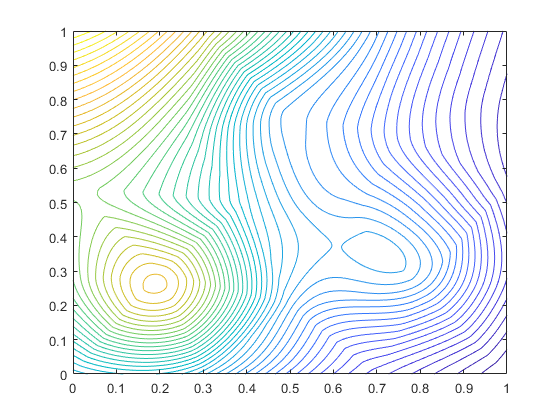
\includegraphics[width=\linewidth]{slike/contour1.png}
\end{subfigure}
\caption*{Contour rešitve z naivno metodo interpolacije.}
\end{figure}

\begin{figure}[H]
\centering
\begin{subfigure}{.9\textwidth}
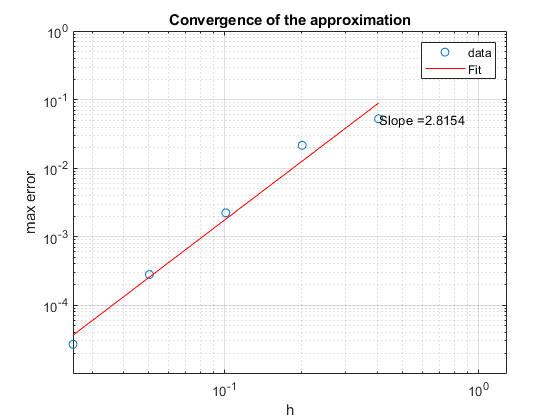
\includegraphics[width=\linewidth]{slike/conv1.png}
\end{subfigure}
\caption*{Konvergenca aproksimacije za naivno metodo.}
\end{figure}


Nadalje poglejmo Foley-Opitz makro element. Izkaže se, da je zlepek spet $C^0$ (po pričakovanjih), red metode pa je višji.

\begin{figure}[H]
\centering
\begin{subfigure}{.9\textwidth}
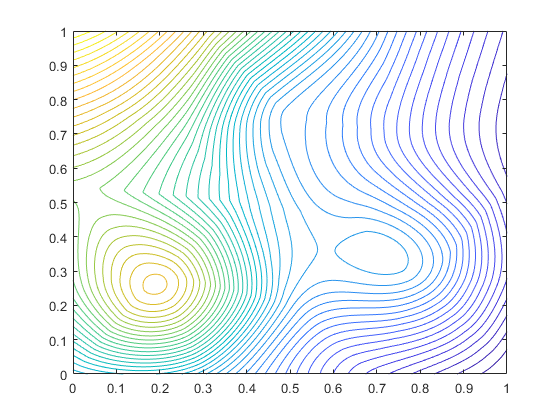
\includegraphics[width=\linewidth]{slike/contour2.png}
\end{subfigure}
\caption*{Contour rešitve za Foley-Opitz.}
\end{figure}

\begin{figure}[H]
\centering
\begin{subfigure}{.9\textwidth}
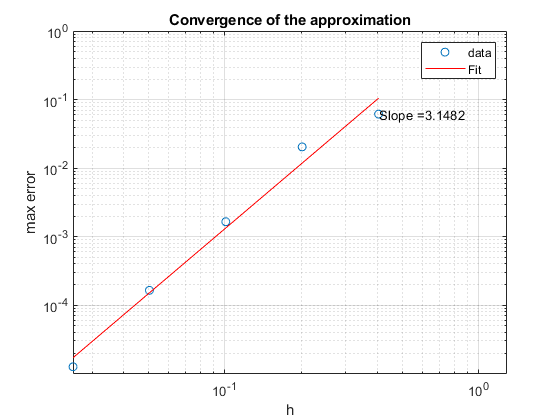
\includegraphics[width=\linewidth]{slike/conv2.png}
\end{subfigure}
\caption*{Konvergenca aproksimacije za Foley-Opitz.}
\end{figure}


Še rezultati za Clough-Tocher. Zlepek naj bi bil $C^1$ kar je za večino stranic res (matrike sem primerjal do tolerance 1e-10), vendar je algoritem našel nekaj stranic, kjer je zlepek ali gladek ali pa sploh nezvezen. Ne vem zakaj se to zgodi, verjetno je nekje v kodi typo, ki enega izmed koeficintov narobe nastavi. Vsaj red metode pa je spet višji kot pri naivni.

\begin{figure}[H]
\centering
\begin{subfigure}{.9\textwidth}
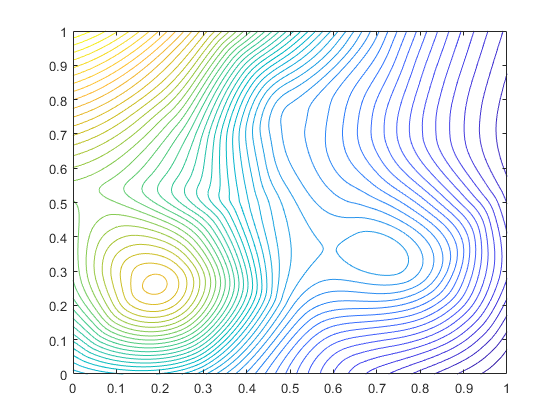
\includegraphics[width=\linewidth]{slike/contour3.png}
\end{subfigure}
\caption*{Contour rešitve za Clough-Tocher.}
\end{figure}

\begin{figure}[H]
\centering
\begin{subfigure}{.9\textwidth}
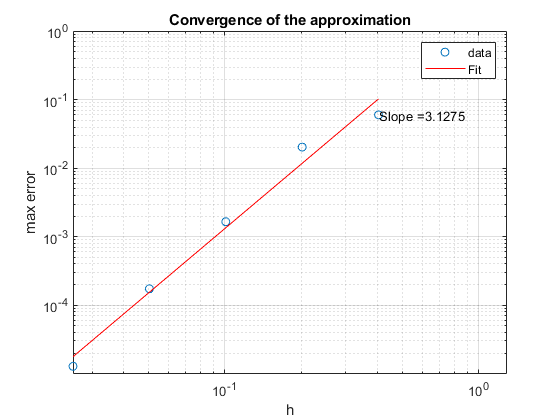
\includegraphics[width=\linewidth]{slike/conv3.png}
\end{subfigure}
\caption*{Konvergenca aproksimacije za Clough-Tocher.}
\end{figure}

\end{document}
